\chapter{Kinematic and dynamic fault sources}\label{cha:Fault-Kinematics-Dynamics}

SPECFEM3D can handle finite fault sources of two kinds:
\begin{enumerate}
\item \emph{Kinematic}: the spatio-temporal distribution of slip rate is
prescribed along the fault surface
\item \emph{Dynamic}: a friction law and initial stresses are prescribed
on the fault, a spontaneous rupture process is computed.
\end{enumerate}

\section{Mesh Generation with Split Nodes}\label{sec:Mesh-Generation-with}

Faults need to be handled in a special way during mesh generation.
A fault surface must lie at the interface between elements (the mesh
must honor the fault surfaces). Moreover, a fault is made of two surfaces
in contact. Each of these two surfaces needs a separate set of nodes.
This approach is known as \textquotedbl{}split nodes\textquotedbl{}.
Currently faults can only be run with \texttt{xdecompose\_mesh} and
\texttt{CUBIT}. \texttt{xmeshfem3D} is not yet ready to handle faults.\\


To facilitate the mesh generation with split nodes in CUBIT, we need
to separate the two fault surfaces by a small distance, effectively
creating a tiny opening of the fault (Figure \ref{fig:examples.splitnodes},
\ref{fig:examples.splitnodes-surfacetrace}). Note that only the interior
of the fault must be opened, its edges must remain closed (except
the edge on the free surface). The fault is automatically closed later
by SPECFEM3D.\\

\noindent
Here is an example CUBIT script to generate a mesh with split nodes
for a buried vertical strike-slip fault:

{\footnotesize
\begin{verbatim}
 reset
 brick x 10 y 10 z 10
 webcut volume all with plane xplane
 webcut volume all with plane yplane
 webcut volume all with plane xplane offset 3
 webcut volume all with plane zplane offset 3
 webcut volume all with plane zplane offset -3
 imprint all
 merge all
 unmerge surf 160
 mesh vol all
 set node constraint off
 node in surf 168 move X 0 Y 0.01 Z 0
 node in surf 160 move X 0 Y -0.01 Z 0
\end{verbatim}
}

\begin{figure}[htbp]
\begin{centering}
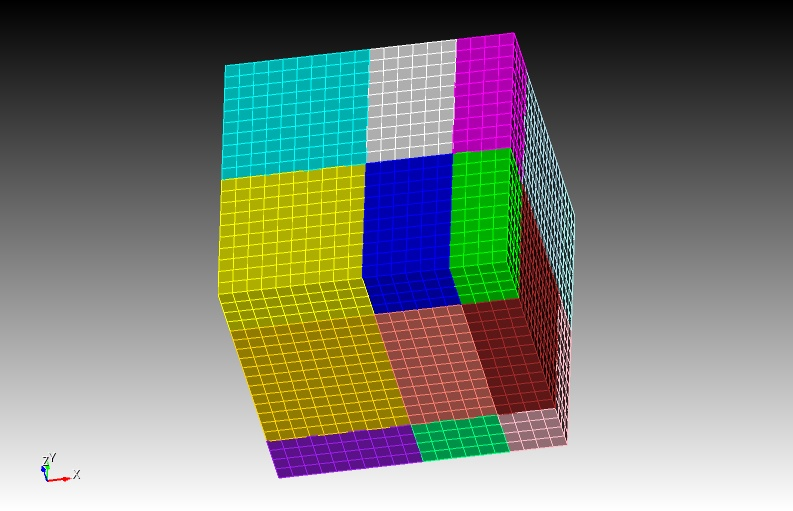
\includegraphics[scale=0.3]{figures/faultmesh.jpg} \\
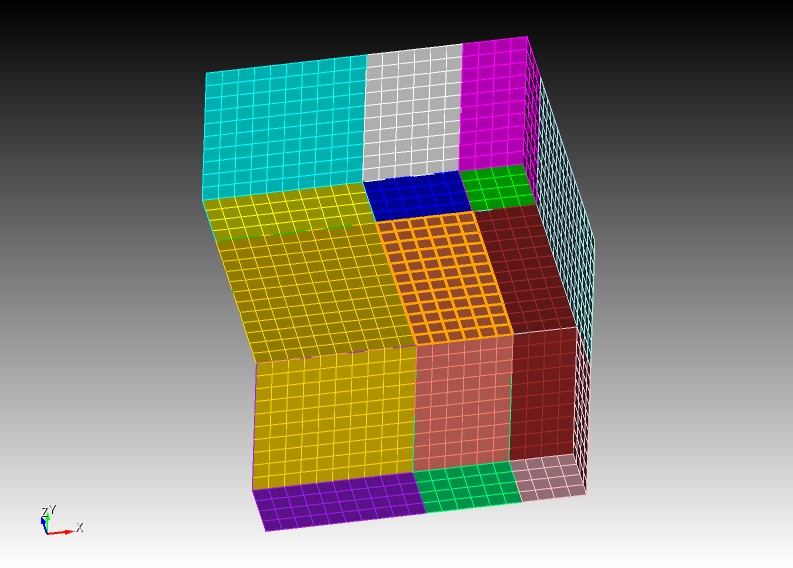
\includegraphics[scale=0.3]{figures/surf168.jpg}
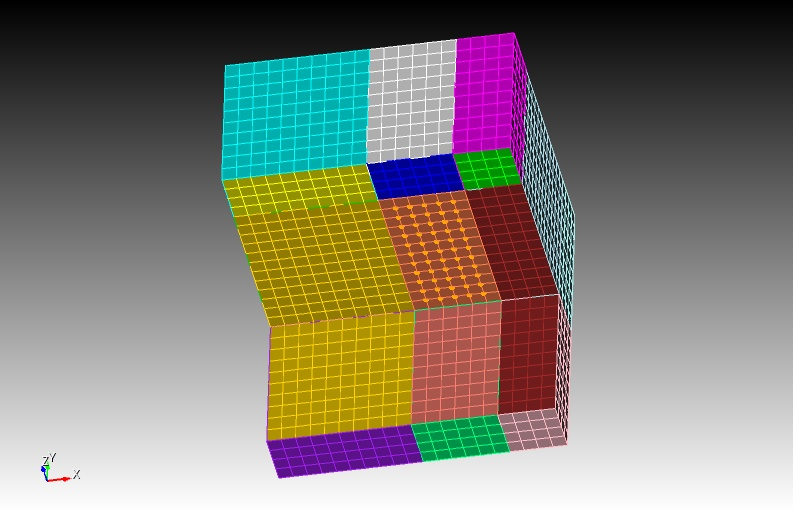
\includegraphics[scale=0.3]{figures/splitnodes.jpg}
\par
\end{centering}
\caption{Screenshots of the CUBIT example for the embedded fault with split
nodes: The entire mesh is decomposed into several volumes bounding
the fault (top), the fault surface 168 is shown as orange squares
(middle) and split nodes of the fault shown as orange dots(bottom).
Note that only interior nodes of the fault are split while those on
the edges of the fault surface are touching each other.}
\label{fig:examples.splitnodes}
\end{figure}

\begin{figure}[htbp]
\begin{centering}
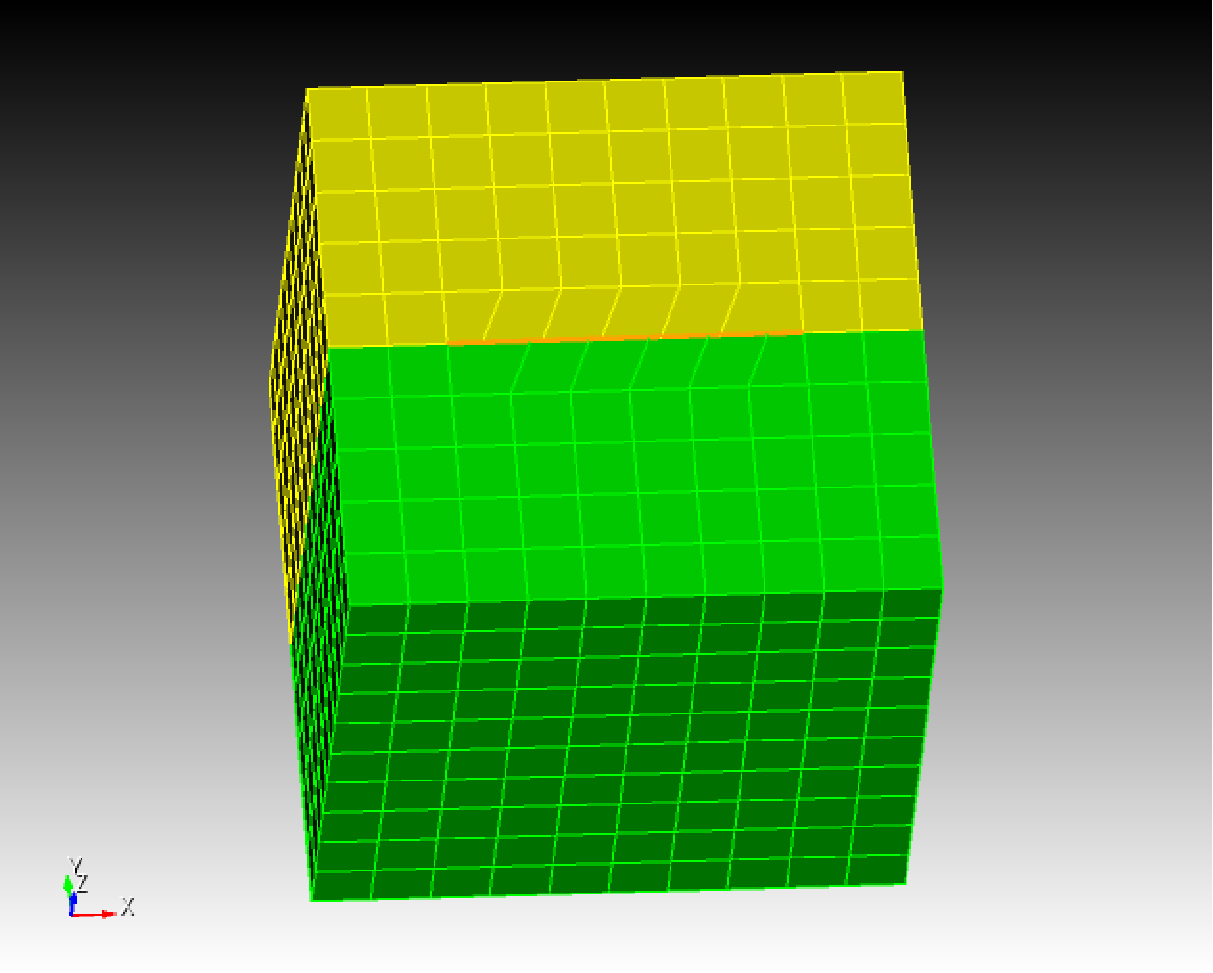
\includegraphics[scale=0.55]{figures/splitnodes_surfacetrace.pdf}
\par
\end{centering}
\caption{Screenshots of a CUBIT example showing split nodes for a fault reaching
the surface. Surface trace of the fault is shown in orange. Note that
the edges of the fault are not split while the interior nodes are
offset by a small distance on either side of the fault}
\label{fig:examples.splitnodes-surfacetrace}
\end{figure}

\noindent
The CUBIT scripts ({*}.jou and {*}.py) in the directory \texttt{EXAMPLES}
generate more complicated meshes. The {*}.py files are Python scripts
that execute CUBIT commands and use the CUBIT-python interface for
SPECFEM3D (see next section). The Python language allows to define
and manipulate variables to parameterize the mesh. Alternatively,
the Python script can call a CUBIT journal file ({*}.jou), which looks
like the example above. Variables can be defined and manipulated there
using the $\mathtt{APREPRO}$ language built in CUBIT.\\

\newpage
\noindent
Note that you should avoid gaps in the list of indices of mesh objects
with the following CUBIT command:

{\footnotesize
\begin{verbatim}
compress ids hex face edge node
\end{verbatim}
}
\noindent
(otherwise you will get a segmentation fault during domain decomposition)


\section{CUBIT-Python Scripts for Faults}

The mesh generated in CUBIT needs to be processed and exported in
a format compatible with SPECFEM3D. This is achieved in the Python
scripts by calling the Python-CUBIT interface functions defined in
the CUBIT directory:
\begin{enumerate}
\item Function $\mathtt{define\_bc}$ (or $\mathtt{boundary\_definition.py}$)
must be called to set up the absorbing boundaries database
\item Function $\mathtt{fault\_input}$ must be called once for each fault
to set up the fault database
\item Function $\mathtt{cubit2specfem3d.export2SPECFEM3D}$ must be called
at the very end of the script to export the mesh in a SPECFEM3D format.
\end{enumerate}
The functions in \#1 and \#3 are for the bulk and are documented in
Section \ref{subsec:Exporting-the-Mesh}. We focus here on \#2:
\begin{description}
\item [{Function:}] $\mathtt{fault\_input}$
\item [{Purpose:}] export a fault mesh database from CUBIT to a SPECFEM3D-compliant
file
\item [{Syntax:}] fault\_input(id\_fault, ids\_surf\_1, ids\_surf\_2)
\item [{Inputs:}]~\end{description}
\begin{itemize}
\item id\_fault integer index assigned to the fault. (The user must number
all the faults, starting at 1, with unit increments)
\item ids\_surf\_1 list of CUBIT ids of all surfaces that form side 1 of
the fault.
\item ids\_surf\_2 list of CUBIT ids of all surfaces that form side 2 of
the fault. (The user must decide which side of the fault is side 1.
This choice affects the sign conventions of fault quantities as explained
in Section \ref{sec:Sign-Convention-for}).\end{itemize}
\begin{description}
\item [{Outputs:}] file $\mathtt{fault\_file\_X.dat}$, where X is the
fault id (id\_fault).
\item [{Example:}] For the example in Section \ref{sec:Mesh-Generation-with}:
\begin{verbatim}
  A1 = [168]
  A2 = [160]
  fault_input(1,A1,A2)
\end{verbatim}
\end{description}

\section{Examples}

The package includes examples, the SCEC benchmark problems:
\begin{itemize}
\item TPV5, a planar vertical strike-slip fault
\item TPV14 and TPV15, vertical strike-slip fault system with a fault branch
\item TPV102 and TPV103, rate-and-state benchmarks
\item TPV22 and TPV23, step-over benchmarks
\item TPV16, heterogenous initial stress
\end{itemize}
and
\begin{itemize}
\item Splay fault models from Wendt et al. (2009)\\

\end{itemize}
Read the documents in the directory \texttt{EXAMPLES/*/description}.
They contain a description of the example and additional instructions
to run it. Visualize the results with the Matlab scripts in the directory
$\mathtt{EXAMPLES/*/post}$


\section{Sign Convention for Fault Quantities}\label{sec:Sign-Convention-for}

During mesh generation, the fault is defined by two surfaces in contact.
Let's denote as \textquotedbl{}\emph{side 1}\textquotedbl{} the SECOND
surface declared by the user in the call to the python function \textquotedbl{}\emph{fault\_input}\textquotedbl{},
and the FIRST surface as \textquotedbl{}\emph{side 2}\textquotedbl{}.
The local coordinate system on the fault is defined as the right-handed
coordinate system defined by (strike, dip, normal), where \textquotedbl{}\emph{normal}\textquotedbl{}
is the normal vector outgoing from side 1, \textquotedbl{}\emph{dip}\textquotedbl{}
is parallel to the along-dip direction pointing downwards, and \textquotedbl{}\emph{strike}\textquotedbl{}
is the horizontal along-strike vector such that the system is right-handed.\\


Slip is defined as displacement on side 2 minus displacement on side
1. In the local coordinate system on the fault, positive along-strike
slip is right-lateral and positive along-dip slip is thrust if side
1 is on the hanging wall (normal faulting if side 1 is on the foot
wall).\\


Traction is defined as the stress induced on side 1 by side 2, which
is the stress tensor times the normal vector outgoing from side 1.
In the local coordinate system on the fault, the normal traction is
negative in compression, positive along-strike traction generates
right-lateral slip and positive along-dip traction generates thrust
slip if side 1 is on the hanging wall (normal faulting if side 1 is
on the foot wall).


\section{Input Files}

Three additional input files are required in the \texttt{DATA/} directory
for dynamic and kinematic faults. They are $\mathtt{Par\_file\_faults}$,
$\mathtt{FAULT\_STATIONS}$ and $\mathtt{input\_file.txt}$ or $\mathtt{rsf\_hete\_input\_file.txt}$(optional).
If the former does not exist, the code assumes that there are no faults.\\

\begin{lyxlist}{00.00.0000}
\item [{\textbf{DATA/Par\_file\_faults}}] contains parameters of the fault.
The first part of this file has a strict format:

\begin{description}
\item [{Line}] 1: Number of faults (NF)
\item [{Lines}] 2 to NF+1: Kelvin Voigt damping (in seconds) for each fault.
(See below how to set this parameter)
\item [{Line}] NF+2: Type of simulation (1=dynamic , 2 = kinematic)
\item [{Line}] NF+3: Number of time steps between updates of the time series
outputs at selected fault points (see DATA/FAULT\_STATIONS), usually
a large number (100s or 1000s). Note that the sampling rate of the
time series is usually much higher.
\item [{Line}] NF+4: Number of time steps between fault snapshot outputs
(quantities at every fault point exported at regular times), usually
a large number (100s or 1000s).
\item [{Line}] NF+5: Slip velocity threshold below which frictional healing
is set (friction coefficient is reset to its static value). If this
value is negative healing is disabled.
\item [{Line}] NF+6: Slip velocity threshold to define the rupture front.
Only used for outputs.
\end{description}

The rest of this file is made of namelist input blocks (see \textquotedbl{}namelist\textquotedbl{}
in a Fortran 9x manual). The input for each fault has the following
sequence (arguments in {[}brackets{]} are optional):

\&\textbf{RUPTURE\_SWITCHES}  /
RATE\_AND\_STATE ,TPV16 ,HETE\_RSF ,TPV10X 

\&\textbf{BEGIN\_FAULT} /

\&\textbf{STRESS\_TENSOR} Sigma = $\sigma_{xx}$,$\sigma_{yy}$,$\sigma_{zz}$,$\sigma_{xy}$,$\sigma_{xz}$,$\sigma_{yz}$ /



\&\textbf{INIT\_STRESS} S1, S2, S3 {[},n1, n2, n3{]} /


followed by (n1+n2+n3) \&\textbf{DIST2D} blocks


\&\textbf{SWF} mus, mud, dc {[}, nmus, nmud, ndc{]} /


\&\textbf{RSF} V0,f0,a,b,L,V\_init,theta\_init,C,StateLaw {[} nV0,nf0,na,nb,nL,nV\_init,ntheta\_init,nC {]} /



followed by (nV0+nf0+na+nb+nL+nV\_init+ntheta\_init+nC) \&\textbf{DIST2D} blocks\\

\begin{lyxlist}{00.00.0000}
\item [{\&\textbf{RUPTURE\_SWITCHES}}] input block sets some switches in the simulation process.
  \begin{description}
    \item [{RATE\_AND\_STATE}] 
         = .TRUE. use rate and state friction,=.FALSE. use slip weakening friction
    \item [{TPV16}]
         =.TRUE turn on heterogeneity fault property input for slip weakening friction from DATA\/input\_file.txt,
         =.FALSE. turn off such feature 
    \item [{HETE\_RSF}]
         =.TRUE. turn on heterogeneity fault property input for rate and state friction 
              using input from DATA\/rsf\_hete\_input\_filr.txt, 
	 =.FALSE. turn off such feature
    \item[{TPV10X}]
         =.TRUE. turn on some ad hoc features for TPV101-104 simulations, a rate strengthening 
	 layer surrounding the rate weakening region. 
	 =.FALSE. turn off such feature
   \end{description}


\item [{\&\textbf{STRESS\_TENSOR}}] input block sets the initial fault stresses 
  by projecting a uniform regional stress field onto the fault plane.So that the 
  tractions $\tau = \sigma : n$ while $n$ is the local norm of the fault plane.
  Sigma =  $\sigma_{xx}$,$\sigma_{yy}$,$\sigma_{zz}$,$\sigma_{xy}$,$\sigma_{xz}$,$\sigma_{yz}$ 
  (in Pa)




\item [{\&\textbf{INIT\_STRESS}}] input block sets the initial fault stresses
relative to the foot-wall side of the fault. Initial stresses are
composed of a constant background value possibly overwritten in prescribed
regions by heterogeneous distributions (see \&\textbf{DIST2D} blocks
below):

\begin{description}
\item [{S1}] = constant background value of along-strike shear stress (positive
in the usual strike direction)
\item [{S2}] = constant background value of along-dip shear (positive is
down-dip, normal faulting)
\item [{S3}] = constant background value of normal stress (negative in
compression)
\item [{n1}] = number of heterogeneous items for along-strike shear stress
{[}default is 0{]}
\item [{n2}] = number of heterogeneous items for along-dip shear stress
{[}default is 0{]}
\item [{n3}] = number of heterogeneous items for normal stress {[}default
is 0{]}
\end{description}
\item [{\&\textbf{SWF}}] input block sets the slip-weakening friction parameters
of the fault:

\begin{description}
\item [{mus}] = constant background value of static friction coefficient
\item [{mud}] = constant background value of dynamic friction coefficient
\item [{dc}] = constant background value of critical slip-weakening distance
\item [{nmus}] = number of heterogeneous items for static friction coefficient
{[}default is 0{]}
\item [{nmud}] = number of heterogeneous items for dynamic friction coefficient
{[}default is 0{]}
\item [{ndc}] = number of heterogeneous items for critical slip-weakening
distance {[}default is 0{]}\\

\end{description}

\item [{\&\textbf{RSF}}] input block sets the rate and state friction parameters
of the fault:

\begin{description}
  \item []
    We refer to the well known rate and state friction formula:
    $$\mu = f_0 + a* log(\frac{v}{v_0}) + b* log(\frac{v_0}{\theta L}))  $$
\item [{V0}] = constant background value of $V_0$
\item [{f0}] = constant background value of $f_0$
\item [{a}] = constant background value of $a$
\item [{b}] = constant background value of $b$
\item [{L}] = constant background value of $L$
\item [{V\_init}] = constant background value of along strike right lateral slip rate at time 0
\item [{theta\_init}] = constant background value of state variable $\theta$ at time 0
\item [{C}] = constant background value of cohesion (in Pa)
\item [{StateLaw}] = 1 or 2. 1 for aging law , 2 for slip law with strong dynamic weakening.
\item [{n**}] = number of heterogeneous items for quantity **
\end{description}



\item [{\&\textbf{DIST2D}}] input blocks modify (overwrite) the value of
a fault parameter by a heterogeneous spatial distribution:


\&\textbf{DIST2D} shape='$\mathtt{square}$', val, xc, yc, zc, l /


$\;$sets a constant value (val) within a cube with center (xc,yc,zc)
and edge size l.


\&\textbf{DIST2D} shape='$\mathtt{rectangle}$', val, xc, yc, zc,
lx, ly, lz /


$\;$sets a constant value (val) within a rectangular prism with center
(xc,yc,zc) and edge sizes (lx,ly,lz).


\&\textbf{DIST2D} shape='$\mathtt{rectangle-taper}$', val, valh,
xc, yc, zc, lx, ly, lz /


$\;$sets a vertical linear gradient within a rectangular prism with
center (xc,yc,zc) and edge sizes (lx,ly,lz). Values vary linearly
as a function of vertical position z between value val at z = zc-lz/2
and value valh at z = zc+lz/2 .


\&\textbf{DIST2D} shape='$\mathtt{circular}$', val, xc, yc, zc, r
/


$\;$sets a constant value (val) within a sphere with center (xc,yc,zc)
and radius r. \\


\end{lyxlist}
\end{lyxlist}

\begin{lyxlist}{00.00.0000}
\item [{\textbf{DATA/FAULT\_STATIONS}}] Stations in the fault plane.


\textbf{Line 1} : number of stations.


\textbf{Line 2 to end}: 5 columns: X, Y, Z (-depth), station name,
fault-id


The fault-id identifies the fault that contains the station. It is
the index of appearance in the faults list after line 2 of Par\_file\_faults

\end{lyxlist}

\begin{lyxlist}{00.00.0000}
\item [{\textbf{DATA/input\_file.txt}}] Heterogeneous stresses and friction for 
linear slip weakening friction
parameters are documented in page 10 of

\begin{lyxlist}{00.00.0000}
\item [{$\mathtt{EXAMPLES/tpv16/description/TPV16\_17\_Description\_v03.pdf}$}]~
\end{lyxlist}

To activate this feature, in Par\_file\_faults name list \&\textbf{RUPTURE\_SWITCHES}, set TPV16=.TRUE..

\end{lyxlist}
\begin{lyxlist}{00.00.0000}
\item [{\textbf{DATA/rsf\_hete\_input\_file.txt}}]  Heterogeneous stresses and friction input for 
  rate and state friction. 
To activate this feature, in Par\_file\_faults name list \&\textbf{RUPTURE\_SWITCHES}, set RSF\_HETE=.TRUE..

  The format of  {\textbf{DATA/rsf\_hete\_input\_file.txt}} is as such, in the first line there are four integers

  that are sequentially documenting the number of divisions along strike, number of divisions along 
  
  dip, cell size along strike , cell size along dip. Then the following N(N=NumberOfDivisionsAlongStrike
  
  * NumberOfDivisionsAlongDip) lines will document the stress and friction properties on the grid.
  
  There are a total of 13 columns.
  \begin{enumerate}
  \item{Column1} = Along strike distance 
  
  \item{Column2} = Along dip distances 

  \item{Column3} = Normal stress(MPa) 

  \item{Column4} = Horizontal right-lateral shear stress(MPa) 

  \item{Column5} = Vertical up-dip shear stress(MPa) 

  \item{Column6} = $V_0$ value in RSF 

  \item{Column7} = $f_0$ value in RSF 
  
  \item{Column8} = a value in RSF  

  \item{Column9} = b value in RSF 
  
  \item{Column10} = L value in RSF 
  
  \item{Column11} = Initial slip velocity 
  
  \item{Column12} = State variable $\theta$ 
  
  \item{Column13} = Cohesion(Pa)  
  \end{enumerate}
  Note that the input grid file do not have to coincide with the mesh. For each fault node on the mesh, they will use the value from the nearest node on the input grid.
\end{lyxlist}


\section{Setting the Kelvin-Voigt Damping Parameter}\label{sec:Setting-the-Kelvin-Voigt}

The purpose of the Kelvin-Voigt viscosity in the dynamic fault solver
is to damp spurious oscillations generated by the fault slip at frequencies
that are too high to be resolved by the mesh. The viscosity $\mathtt{eta}$
(in seconds) depends on the size of the elements on the fault. Here
is how to set it:
\begin{enumerate}
\item Determine the average linear size of the elements on the fault plane,
$\mathtt{h\_fault}$. Usually this value is prescribed by the user
during mesh generation. Otherwise it can be found by inspection of
the mesh inside the CUBIT GUI.
\item Use the Matlab function $\mathtt{utils/critical\_timestep.m}$ to
compute\\
 $\mathtt{dtc\_fault}=\mathtt{critical\_timestep\left(c_{p},h\_fault,ngll\right)}$.
\\
This is the critical time step in an elastic medium for a hypothetical
element of cubic shape with size equal to $\mathtt{h\_fault}$.
\item Set $\mathtt{eta}$ in $\mathtt{Par\_file\_faults}$ to (0.1 to 0.3)$\ensuremath{\times}\mathtt{dtc\_fault}$.
A larger $\mathtt{eta}$ damps high-frequencies more aggressively
but it might also affect lower frequencies and rupture speed.
\end{enumerate}
Viscosity reduces numerical stability: the critical timestep in a
simulation with Kelvin-Voigt damping needs to be smaller than that
in a purely elastic simulation. Here is how to set the time step accordingly:
\begin{enumerate}
\item Run a test simulation without viscosity ($\mathtt{eta}$=0 and only
a few time steps)
\item Look for the \textquotedbl{}maximum suggested time step\textquotedbl{}
in \texttt{OUTPUT\_FILES/output\_mesher.txt}. This is the critical
timestep of a purely elastic simulation, $\mathtt{dtc\_bulk}$.
\item Reset the timestep of the simulation with a Kelvin-Voigt material
to a value smaller than\\
 $\mathtt{dtc\_kv}=\mathtt{eta}\left(\sqrt{1+\mathtt{dtc\_bulk^{2}}/\mathtt{eta^{2}}}-1\right)$
\end{enumerate}
Note that in general $\mathtt{dtc\_bulk}$ is smaller than $\mathtt{dtc\_fault}$,
because elements off the fault might be smaller or more distorted
than element faces on the fault.


\section{Output Files }

Several output files are saved in \texttt{OUTPUT\_FILES/}:\\

\begin{enumerate}
\item Seismograms for each station on the fault plane given in \texttt{DATA/FAUL\_STATIONS}.
One output file is generated for each station, named after the station.
The files are ascii and start with a header (22 lines long) followed
by a data block with the following format, one line per time sample:\\



Column 1 = Time (s)


Column 2 = horizontal right-lateral slip (m)


Column 3 = horizontal right-lateral slip rate (m/s)


Column 4 = horizontal right-lateral shear stress (MPa)


Column 5 = vertical up-dip slip (m)


Column 6 = vertical up-dip slip rate (m/s)


Column 7 = vertical up-dip shear stress (MPa)


Column 8 = normal stress (MPa)\\



The stresses are relative to the footwall side of the fault (this
convention controls their sign, but not their amplitude). Slip is
defined as displacement of the hanging wall relative to the footwall.

\item Seismograms at stations in the bulk (out of the fault plane) given
in \texttt{DATA/STATIONS}.
\item Rupture time files are named $\mathtt{Rupture\_time\_FAULT}$-$\mathtt{id}$.
One file is generated for each fault. The files are ascii and start
with a header (12 lines long) followed by a data block with the following
format, one line per fault node:


Column 1 = horizontal coordinate, distance along strike (m)


Column 2 = vertical coordinate, distance down-dip (m)


Column 3 = rupture time (s)

\item Fault quantities (slip, slip rate, stresses, etc) at regular times
are stored in binary data files called $\mathtt{Snapshot\#it\#.bin}$,
where \#it\# is the timestep number. These can be read in Matlab with
the function $\mathtt{utils/FSEM3D\_snapshot.m}$
\end{enumerate}

\section{Post-processing and Visualization}

Some Matlab functions for post-processing and visualization are included
in directory $\mathtt{utils}$. The functions are internally documented
(see their matlab help).\\


\texttt{FSEM3D\_snapshot} reads a fault data snapshot\\

\noindent
The directories \texttt{EXAMPLES/*/post} contain additional Matlab
scripts to generate figures specific to each example.

